% !TEX program = xelatex
\documentclass[zihao=-4,a4paper]{ctexart}
\usepackage{fontspec}
\usepackage{xeCJK}
\usepackage{amsmath,amssymb,bm}
\usepackage{graphicx}
\usepackage{listings}
\usepackage{xcolor}
\usepackage{float}
\usepackage{enumitem}
\usepackage{caption}
\usepackage{booktabs,tabularx}
\usepackage{array}
\usepackage{changepage} % 用于调整局部正文的左右边距
\usepackage{algorithm}
\usepackage{algpseudocode}
\usepackage{pdfpages}
\setmonofont{Consolas}   % 设置等宽字体为 Consolas
\setCJKmainfont{SimSun}[AutoFakeBold=2.5]
\usepackage{hyperref}
% 页面布局
\usepackage[
  top    = 1.7cm,
  left   = 1.7cm,
  right  = 1.7cm,
  bottom = 2.7cm,
  footskip = 1cm
]{geometry}
\linespread{1.5}
% 提供 current page text area 节点
\usepackage{tikzpagenodes}
\usetikzlibrary{calc}            % 用于计算坐标
\usepackage{fancyhdr}
% ==============================
% 全局变量: 存储版心宽度
% ==============================
\newlength{\myTextWidth}
\newcommand{\calcTextWidth}{%
  \path let \p1=(current page text area.east), \p2=(current page text area.west) in 
    \pgfextra{\pgfmathsetlength{\myTextWidth}{\x1-\x2}};
}

% ==============================
% 背景画线逻辑
% ==============================
\newif\ifdrawbackground  % 定义背景绘制开关
\drawbackgroundtrue      % 默认开启背景绘制
\AddToHook{shipout/background}{%
  \ifdrawbackground %只有开关开启时才绘制背景
  \tikz[remember picture, overlay]{%
    
    % 定义上下外扩的距离(和表格撑开的距离保持一致)
    \def\vpad{0.8em} 

    % --- 所有页: 底部横线 (向下偏移 \vpad) ---
    \draw[line width=1pt] 
      ([yshift=-\vpad]current page text area.south west) -- 
      ([yshift=-\vpad]current page text area.south east);

    \ifnum\value{page}=10
      % --- 第一页: 绘制 2x6 表格边框 ---
      \def\innerLineWidth{0.8pt}
      \def\outerLineWidth{1pt}

      % 1. 上横线 (表格节点已通过 inner ysep 撑开, 直接画)
      \draw[line width=\outerLineWidth] 
        (title-bottom-mark -| current page text area.west) -- 
        (title-bottom-mark -| current page text area.east);

      % 2. 下横线 (同上)
      \draw[line width=\outerLineWidth] 
        (table-bottom-mark -| current page text area.west) -- 
        (table-bottom-mark -| current page text area.east);

      % 3. 中间横线 (自动居中)
      \draw[line width=\innerLineWidth] 
        ($(title-bottom-mark -| current page text area.west)!0.5!(table-bottom-mark -| current page text area.west)$) -- 
        ($(title-bottom-mark -| current page text area.east)!0.5!(table-bottom-mark -| current page text area.east)$);

      % 4. 左右外框竖线 (从表格顶部一直到页底, 页底向下偏移 \vpad)
      \draw[line width=\outerLineWidth] 
        (title-bottom-mark -| current page text area.west) -- 
        ([yshift=-\vpad]current page text area.south west);
      \draw[line width=\outerLineWidth] 
        (title-bottom-mark -| current page text area.east) -- 
        ([yshift=-\vpad]current page text area.south east);

      % 5. 内部竖线 (5条)
      \foreach \i in {1,2,...,5} {
        \pgfmathsetmacro{\pos}{\i/6}
        \draw[line width=\innerLineWidth]
          ($(title-bottom-mark -| current page text area.west)! \pos !(title-bottom-mark -| current page text area.east)$) --
          ($(table-bottom-mark -| current page text area.west)! \pos !(table-bottom-mark -| current page text area.east)$);
      }

    \else
      % --- 后续页: 标准四周边框 (上下各外扩 \vpad) ---
      % 顶部横线向上偏移
      \draw[line width=1pt] ([yshift=\vpad]current page text area.north west) -- ([yshift=\vpad]current page text area.north east);
      % 左右竖线跟随上下偏移
      \draw[line width=1pt] ([yshift=\vpad]current page text area.north west) -- ([yshift=-\vpad]current page text area.south west);
      \draw[line width=1pt] ([yshift=\vpad]current page text area.north east) -- ([yshift=-\vpad]current page text area.south east);
    \fi
  }%
  \fi
}


\pagestyle{fancy}
\fancyhf{}
\fancyfoot[C]{\thepage}
\renewcommand{\headrulewidth}{0pt}

% 直接使用 \textwidth 计算列宽
% ==============================
% \textwidth/6 保证精确6等分, 减去 2\tabcolsep 扣除单元格自带的左右边距
\newcolumntype{C}{>{\raggedright\arraybackslash}p{\dimexpr\textwidth/6-2\tabcolsep\relax}}

% 自定义命令: 在当前位置画一条贯穿全宽的横线
% ==============================
\newcommand{\addhline}{%
  \par
  \noindent
  
\begin{tikzpicture}[remember picture, overlay]
    % (0,0) 代表当前文字所在的高度
    % current page text area.west 代表版心最左侧
    % |- 符号表示: 取左边的 X 坐标, 取右边的 Y 坐标
    \draw[line width=1pt] 
      (current page text area.west |- 0,0) -- 
      (current page text area.east |- 0,0);
  \end{tikzpicture}\par
}

\newcommand{\dd}{\mathop{}\!\mathrm{d}}
\newcommand{\myS}{14}
\newcommand{\myt}{0.21}

% MATLAB 代码风格
\definecolor{matlabgreen}{rgb}{0,0.6,0}
\definecolor{matlabgray}{rgb}{0.5,0.5,0.5}
\definecolor{matlabpurple}{rgb}{0.58,0,0.82}
\definecolor{matlabbg}{rgb}{0.95,0.95,0.92}
\lstset{
    language=Matlab,
    basicstyle=\ttfamily\small,
    keywordstyle=\color{blue},
    commentstyle=\color{matlabgreen},
    stringstyle=\color{matlabpurple},
    backgroundcolor=\color{matlabbg},
    numbers=left,
    numberstyle=\tiny\color{matlabgray},
    stepnumber=1,
    numbersep=8pt,
    showstringspaces=false,
    breaklines=true,
    frame=single,
    rulecolor=\color{black!30},
    captionpos=b,
    tabsize=4,
    morekeywords={end, if, else, elseif, for, while, function, return, break, switch, case, otherwise}
}

\begin{document}
\setcounter{page}{10}
\begin{center}
  \zihao{-2}\bfseries 数值分析实践报告(四)
\end{center}

% --- 表格内容区 ---
\noindent
\begin{tikzpicture}[remember picture]
  % 将整个 tabular 放入一个 TikZ 节点中, 彻底屏蔽 LaTeX 段落间距的干扰
  \node[anchor=north west, inner sep=0pt, outer sep=0pt] (header-table) at (0,0) {%
    \renewcommand{\arraystretch}{1.8}% 增加行高
    \begin{tabular}{CCCCCC} 
      姓\quad 名 & VesperaZephyr & 班\quad 级 & \small 数学与应用数学 & 报告评分 & \\
      学\quad 号 & 114514 & 地点/机号 &  & 指导教师 & 
    \end{tabular}%
  };
  
  % 自动获取这个表格真实的左上角和左下角坐标, 传给背景画线
  \coordinate (title-bottom-mark) at (header-table.north west);
  \coordinate (table-bottom-mark) at (header-table.south west);
\end{tikzpicture}

\setlength{\leftskip}{1em}
\setlength{\rightskip}{1em}

% 实验名称
\noindent{\bfseries 一、实验项目名称: 最小二乘拟合及其应用}

\addhline

\noindent{\bfseries 二、实验目的: }
\begin{enumerate}[rightmargin=0.5cm]
  \item 理解最小二乘法的基本原理：掌握通过最小化残差平方和来拟合线性模型参数的数学思想, 理解法方程组的推导过程。
  \item 掌握参数的计算方法：根据实验数据, 熟练运用最小二乘法计算线性回归模型中的参数。
  \item 培养工程问题建模能力：学会将工程中的问题转化为数学模型, 并运用数值方法求解。
  \item 学会模型评价与预测：掌握误差的计算方法, 能够评估拟合优度；并利用拟合模型进行工程预测。
  \item 提升编程与数据可视化能力：能够使用 Python(或其它语言)实现最小二乘算法, 绘制原始数据点、拟合曲线、残差分析图, 直观展示拟合效果。
  \item 培养误差分析与批判性思维：通过残差分析和模型局限性讨论, 认识拟合模型的适用条件, 理解实际工程中数据误差的来源及其对预测结果的影响。
\end{enumerate}

\addhline

\noindent{\bfseries 实验内容: }

某矿山机械厂对一批球磨机衬板进行磨损寿命试验。衬板在服役过程中, 其厚度磨损量随时间逐渐增加。为制定合理的衬板更换周期, 工程师记录了连续运行时间 $t$(单位：天)与对应的累计磨损量 $h$(单位：mm), 数据如下：

\[
\begin{array}{c|cccccccc}
\text{时间 } t & 5 & 10 & 15 & 20 & 25 & 30 & 35 & 40 \\
\hline
\text{磨损量 } h & 0.8 & 1.6 & 2.3 & 3.1 & 3.8 & 4.5 & 5.2 & 6.0
\end{array}
\]

根据摩擦学理论, 在稳定磨损阶段, 磨损量与时间通常呈线性关系：
\[
h(t)=a+b\,t
\]
其中：$a$ 为初始磨损量(mm), $b$ 为磨损速率(mm/天)。

\addhline

\noindent{\bfseries 四、模型构建}

对于给定的 $m$ 组观测数据 $(t_i, h_i),\ i=1,2,\dots,m$, 假设磨损量 $h$ 与时间 $t$ 满足线性关系: 
\[
h = a + bt,
\]
记拟合值为 $\hat{h}_i = a + bt_i$, 残差 $e_i = h_i - \hat{h}_i$. 

采用最小二乘准则, 定义误差函数为残差平方和: 
\begin{equation}
Q(a,b) = \sum_{i=1}^{m} e_i^2 = \sum_{i=1}^{m} (h_i - a - b t_i)^2.
\end{equation}
目标是求参数 $a,b$ 使 $Q(a,b)$ 最小. 分别对 $a$ 和 $b$ 求偏导并令其为零: 
\[
\begin{cases}
\dfrac{\partial Q}{\partial a} = -2\sum\limits_{i=1}^{m}(h_i - a - bt_i) = 0, \\[8pt]
\dfrac{\partial Q}{\partial b} = -2\sum\limits_{i=1}^{m}(h_i - a - bt_i)t_i = 0.
\end{cases}
\]
整理得法方程组(正规方程): 
\begin{equation}
\begin{cases}
m a + \left(\sum\limits_{i=1}^{m} t_i\right) b = \sum\limits_{i=1}^{m} h_i, \\[8pt]
\left(\sum\limits_{i=1}^{m} t_i\right) a + \left(\sum\limits_{i=1}^{m} t_i^2\right) b = \sum\limits_{i=1}^{m} t_i h_i.
\end{cases}
\end{equation}
记
\[
S_t = \sum t_i,\quad S_h = \sum h_i,\quad S_{tt} = \sum t_i^2,\quad S_{th} = \sum t_i h_i,\quad \bar{t}=\frac{S_t}{m},\ \bar{h}=\frac{S_h}{m},
\]
则参数的最小二乘估计为: 
\begin{equation}
b = \frac{m S_{th} - S_t S_h}{m S_{tt} - S_t^2} = \frac{\sum (t_i-\bar{t})(h_i-\bar{h})}{\sum (t_i-\bar{t})^2},
\end{equation}
\begin{equation}
a = \bar{h} - b \bar{t}.
\end{equation}

\noindent{\bfseries 五、模型求解}

针对本题, 算法步骤为:
\begin{center}
\begin{minipage}{0.9\textwidth}
\begin{algorithm}[H]
\caption{最小二乘法线性回归拟合及预测}
\begin{algorithmic}[1]
\Require 观测天数 $t_i$ 和磨损量 $h_i$, $i=1,\dots,m$, 目标磨损量 $h_{\text{target}}=8.0$(mm)
\Ensure 拟合参数 $a$(初始磨损量)、$b$(磨损速率), 决定系数 $R^2$, 预测天数 $t_{\text{predict}}$
\State 计算统计量：
\State \quad $S_t = \sum_{i=1}^{m} t_i$
\State \quad $S_h = \sum_{i=1}^{m} h_i$
\State \quad $S_{tt} = \sum_{i=1}^{m} t_i^2$
\State \quad $S_{th} = \sum_{i=1}^{m} t_i h_i$
\State 估计回归参数：
\State \quad $b = \dfrac{m S_{th} - S_t S_h}{m S_{tt} - S_t^2}$
\State \quad $a = \bar{h} - b \bar{t}$, 其中 $\bar{h}=S_h/m$, $\bar{t}=S_t/m$
\State 输出拟合方程：$h = a + b t$
\State 计算拟合值 $\hat{h}_i = a + b t_i$, 残差 $e_i = h_i - \hat{h}_i$
\State 计算残差平方和：$Q = \sum_{i=1}^{m} e_i^2$
\State 计算总平方和：$S_{\text{tot}} = \sum_{i=1}^{m} (h_i - \bar{h})^2$
\State 计算决定系数：$R^2 = 1 - Q / S_{\text{tot}}$
\State 输出 $Q$ 和 $R^2$
\State 预测磨损量达到 $h_{\text{target}}$ 所需天数：
\State \quad $t_{\text{predict}} = \dfrac{h_{\text{target}} - a}{b}$
\State 输出 $t_{\text{predict}}$
\end{algorithmic}
\end{algorithm}
\end{minipage}
\end{center}

编写Matlab程序求解, 代码文件为\verb|least_squares_fitting.m|, 运行结果见表\ref{tab:least_squares_results}.

\addhline
\noindent{\bfseries 六、实验结果}

\noindent{\bfseries 6.1 代码结果}

代码文件为\verb|least_squares_fitting.m|, 运行结果见表\ref{tab:least_squares_results}:
\begin{table}[htbp]
\centering
\caption{线性回归拟合结果}
\label{tab:least_squares_results}
\begin{tabular}{cc}
\toprule
\text{拟合方程} & $h = 0.1071 + 0.1469\,t$ \\
\text{初始磨损量 } $a$ & $0.1071\ \text{mm}$ \\
\text{磨损速率 } $b$ & $0.1469\ \text{mm/天}$ \\
\text{残差平方和 } $Q$ & $0.008690$ \\
\text{决定系数 } $R^2$ & $0.999617$ \\
\text{预测达到 8.0 mm 的服役天数} & $53.73\ \text{天}$ \\
\bottomrule
\end{tabular}
\end{table}

根据表\ref{tab:least_squares_results}的结果分析如下:
\begin{itemize}
    \item 拟合得到的线性方程为 $h(t) = 0.1071 + 0.1469\,t$. 
    \item 残差平方和 $Q \approx 0.0087$, 数值极小, 说明回归直线对数据的整体偏差很小. 
    \item 决定系数 $R^2 = 0.9996$, 非常接近 $1$, 表明模型能够解释 $99.96\%$ 的磨损量变异, 线性关系极其显著, 模型可靠性极高. 
    \item 预测当磨损量达到报废标准 $8.0$ mm 时, 衬板的服役时间约为 $53.73$ 天. 
\end{itemize}

在\verb|least_squares_fitting.m|的基础上, 进行可视化, 绘制残差图, 进一步分析拟合效果与模型的适用性. 代码文件为\verb|least_squares_fitting_visualization.m|, 运行结果见下:
\begin{table}[H]
\centering
\caption{线性回归残差}
\label{tab:residuals}
\begin{tabular}{cc}
\toprule
$t$ / 天 & $e$ / mm \\
\midrule
 5 & $-0.0417$ \\
10 &  $0.0238$ \\
15 & $-0.0107$ \\
20 &  $0.0548$ \\
25 &  $0.0202$ \\
30 & $-0.0143$ \\
35 & $-0.0488$ \\
40 &  $0.0167$ \\
\bottomrule
\end{tabular}
\end{table}

\begin{figure}[H]
\centering
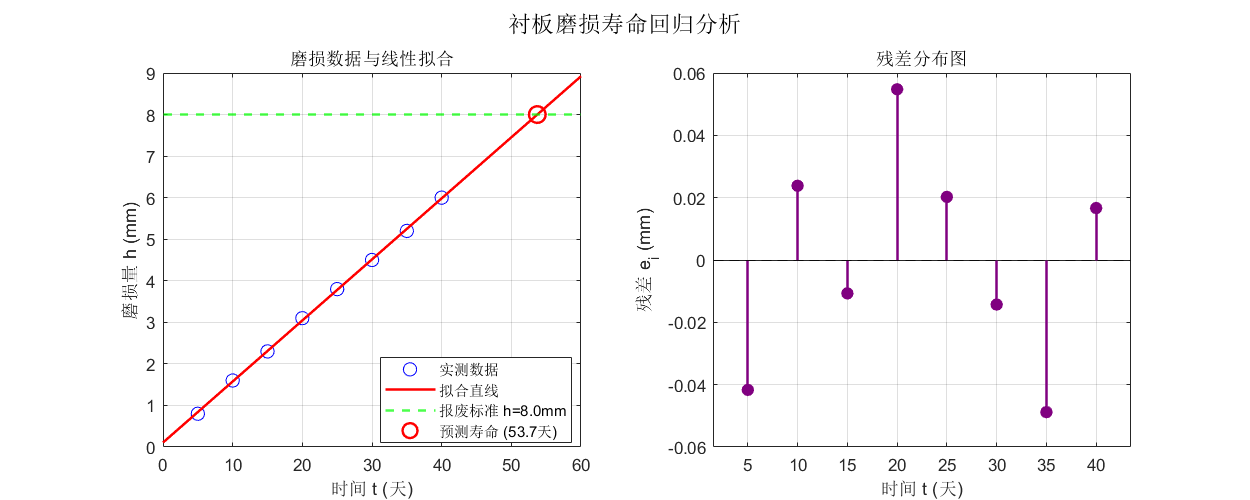
\includegraphics[width=0.95\textwidth]{衬板磨损寿命回归分析.png}
\caption{衬板磨损寿命回归分析}
\label{fig:result}
\end{figure}

从残差图可见, 残差在零线附近随机分布, 未呈现弯曲或异方差趋势, 进一步验证了线性模型的适用性. 
\end{document}
